% =====================================================================
%  Laboratorio de la Sesión 5: DBSCAN, HDBSCAN y agrupamiento espectral
%  en formas no convexas
%  Se incluye desde Sesion5-Densidad_Espectral.tex con % =====================================================================
%  Laboratorio de la Sesión 5: DBSCAN, HDBSCAN y agrupamiento espectral
%  en formas no convexas
%  Se incluye desde Sesion5-Densidad_Espectral.tex con % =====================================================================
%  Laboratorio de la Sesión 5: DBSCAN, HDBSCAN y agrupamiento espectral
%  en formas no convexas
%  Se incluye desde Sesion5-Densidad_Espectral.tex con % =====================================================================
%  Laboratorio de la Sesión 5: DBSCAN, HDBSCAN y agrupamiento espectral
%  en formas no convexas
%  Se incluye desde Sesion5-Densidad_Espectral.tex con \input{Laboratorio}
%  El mismo código, ejecutado, está en laboratorio_densidad_espectral.ipynb
% =====================================================================
\section{Laboratorio: densidad y espectral en formas no convexas}
% =====================================================================

\begin{frame}[fragile]{Paso 1: los datos}
\begin{lstlisting}
import numpy as np, pandas as pd
from sklearn.datasets import make_moons, make_circles, make_blobs
from sklearn.cluster import KMeans, DBSCAN, HDBSCAN, SpectralClustering
from sklearn.neighbors import NearestNeighbors
from sklearn.metrics import adjusted_rand_score

Xm, ym = make_moons(500, noise=0.07, random_state=0)
Xc, yc = make_circles(500, factor=0.45, noise=0.05, random_state=0)
Xb, yb = make_blobs([150, 150, 250], centers=[[0, 0], [1.3, 0], [4.5, 3]],
                    cluster_std=[0.2, 0.2, 1.0], random_state=0)
ruido = np.random.default_rng(0).uniform([-2, -2], [8, 7], (50, 2))
Xd, yd = np.r_[Xb, ruido], np.r_[yb, -np.ones(50, int)]   # el ruido tiene etiqueta -1
datos = {"Lunas": (Xm, ym), "Círculos": (Xc, yc), "Densidades": (Xd, yd)}
\end{lstlisting}
  {\small Las etiquetas verdaderas sólo se usan para evaluar con el ARI; el ruido cuenta como una clase más.}
\end{frame}

\begin{frame}{Paso 1: los tres conjuntos}
  \centering
  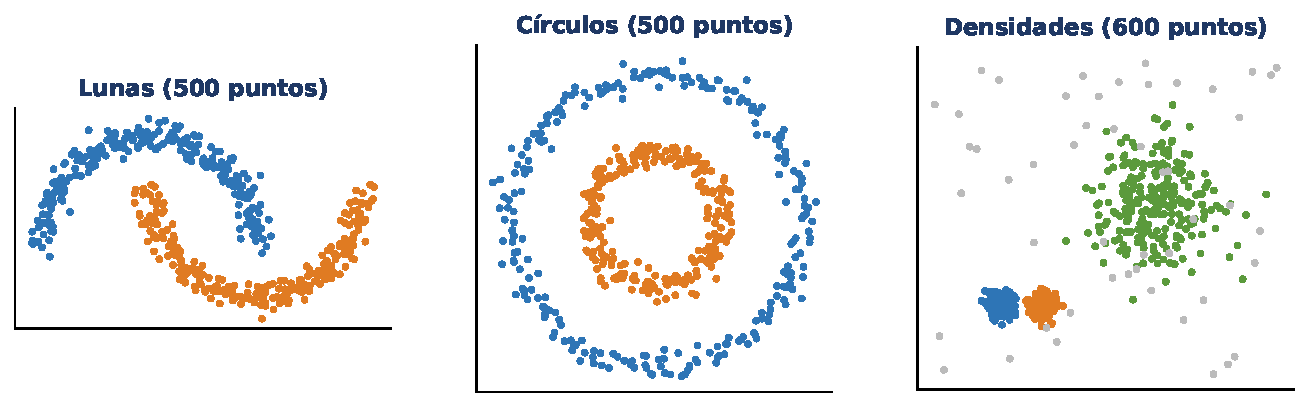
\includegraphics[width=0.95\textwidth]{lab_datos}
  \begin{itemize}
    \item \textbf{Lunas}: dos grupos entrelazados, no convexos.
    \item \textbf{Círculos}: un grupo rodea al otro; ningún centro los separa.
    \item \textbf{Densidades}: dos grupos densos y pegados, uno disperso, y 50 puntos de ruido uniforme.
  \end{itemize}
\end{frame}

\begin{frame}[fragile]{Paso 2: elegir $\eps$ para DBSCAN}
\begin{lstlisting}
for nombre, (X, y) in datos.items():
    d = np.sort(NearestNeighbors(n_neighbors=10).fit(X).kneighbors(X)[0][:, -1])
    plt.plot(d)    # grafica de k-distancia con min_samples = 10
\end{lstlisting}
  \centering
  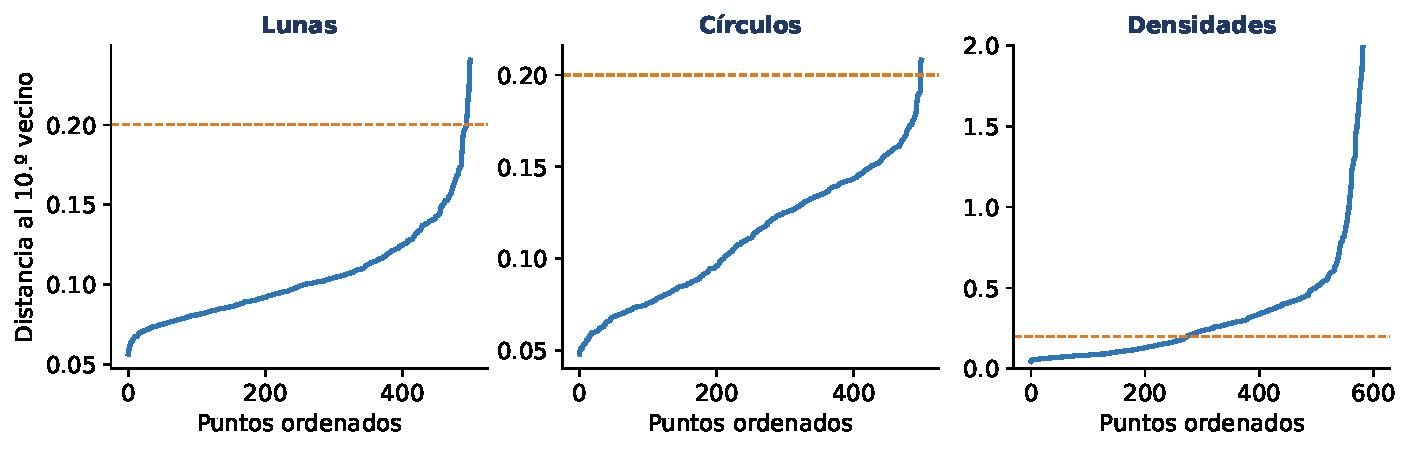
\includegraphics[width=0.9\textwidth]{lab_k_distancia}
  \begin{itemize}
    \item En lunas y círculos el codo está cerca de 0.2: se usa $\eps = 0.2$ y \texttt{min\_samples} $= 10$.
    \item En densidades la curva sube de forma gradual: no hay un codo claro, señal de que las
          densidades son distintas.
  \end{itemize}
\end{frame}

\begin{frame}[fragile]{Paso 3: DBSCAN con densidades distintas}
\begin{lstlisting}
X, y = datos["Densidades"]
for eps in np.arange(0.1, 1.01, 0.05):
    z = DBSCAN(eps=eps, min_samples=10).fit_predict(X)
    print(round(eps, 2), adjusted_rand_score(y, z))
\end{lstlisting}
  \begin{columns}[c]
    \column{0.48\textwidth}
    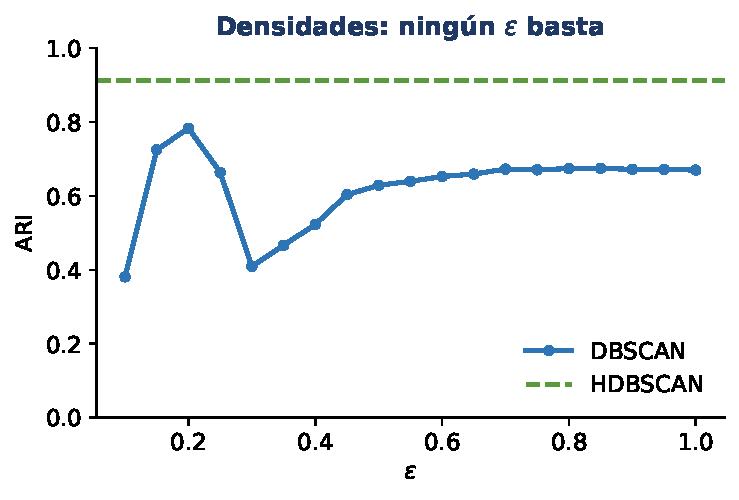
\includegraphics[width=\textwidth]{lab_barrido}
    \column{0.5\textwidth}
    \small
    \begin{itemize}
      \item El mejor DBSCAN obtiene ARI 0.78, con $\eps = 0.2$: separa los dos grupos densos,
            pero 236 de los 250 puntos del disperso quedan como ruido.
      \item Con $\eps \ge 0.35$ los dos densos se unen en un grupo; el disperso aparece, pero con parte de sus puntos como ruido.
      \item HDBSCAN, con \texttt{min\_cluster\_size} $=15$ y sin elegir $\eps$, obtiene 0.91.
    \end{itemize}
  \end{columns}
\end{frame}

\begin{frame}[fragile]{Paso 4: los cuatro métodos en los tres conjuntos}
\begin{lstlisting}
for nombre, (X, y) in datos.items():
    k = len(set(y) - {-1})
    modelos = {"k-medias": KMeans(k, n_init=10, random_state=0),
               "DBSCAN": DBSCAN(eps=0.2, min_samples=10),
               "HDBSCAN": HDBSCAN(min_cluster_size=15),
               "Espectral": SpectralClustering(k, affinity="nearest_neighbors",
                                               n_neighbors=10, random_state=0)}
    for metodo, modelo in modelos.items():
        z = modelo.fit_predict(X)
        print(nombre, metodo, round(adjusted_rand_score(y, z), 2), (z == -1).sum())
\end{lstlisting}
  \vspace{4pt}
  \centering
  \small
  \begin{tabular}{@{}lcccc@{}}
    \toprule
    \textbf{ARI} & \textbf{k-medias} & \textbf{DBSCAN} & \textbf{HDBSCAN} & \textbf{Espectral}\\
    \midrule
    Lunas      & 0.24 & 1.00 & 1.00 & 1.00 \\
    Círculos   & 0.00 & 1.00 & 1.00 & 1.00 \\
    Densidades & 0.46 & 0.78 & 0.91 & 0.85 \\
    \bottomrule
  \end{tabular}
\end{frame}

\begin{frame}{Paso 4: los resultados}
  \begin{columns}[c]
    \column{0.58\textwidth}
    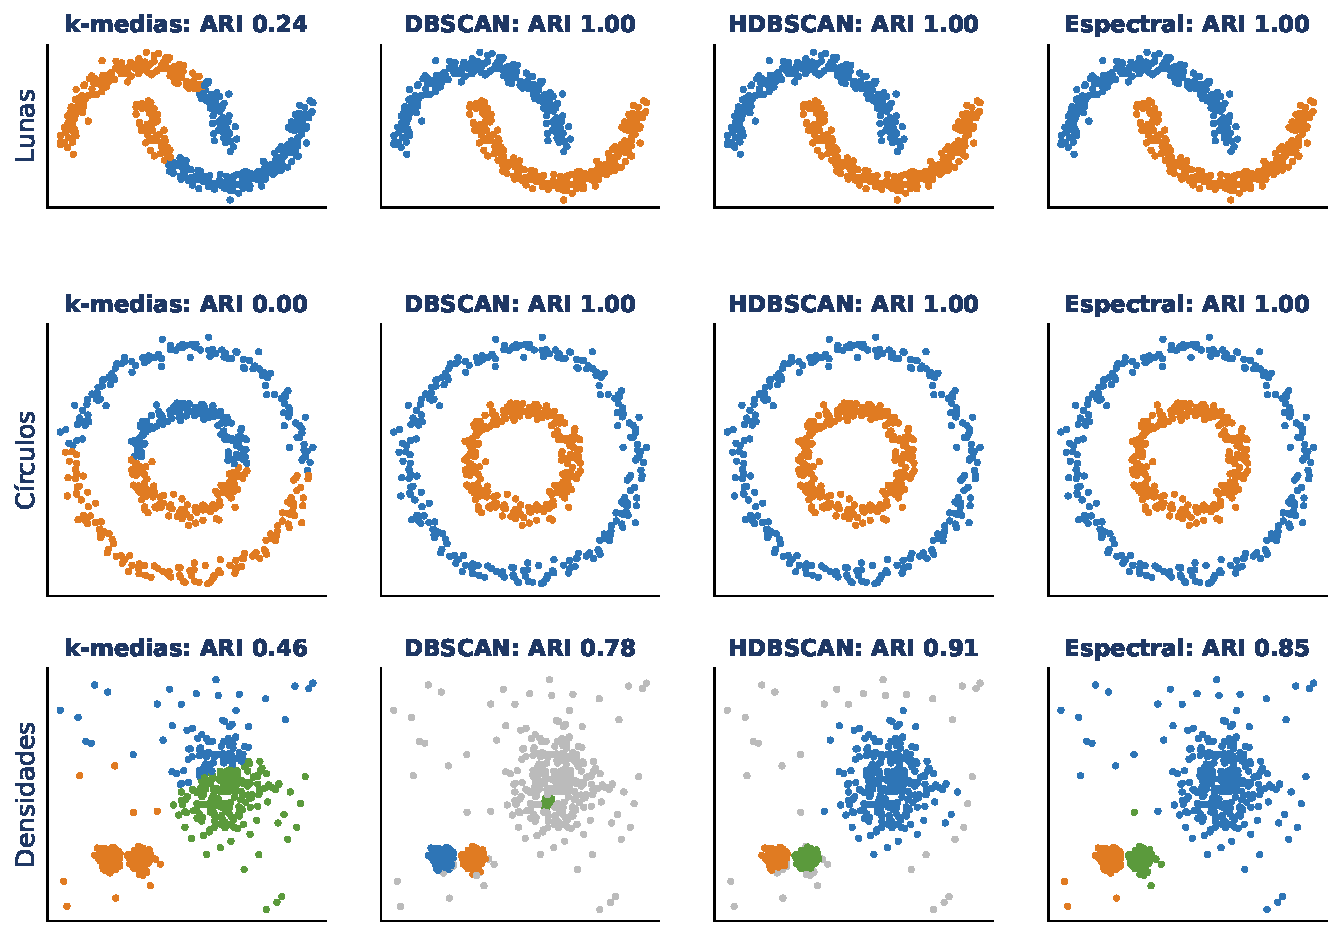
\includegraphics[width=\textwidth]{lab_comparacion}
    \column{0.4\textwidth}
    \small
    \begin{itemize}
      \item Lunas y círculos: los tres métodos no convexos aciertan; k-medias corta las formas.
      \item Densidades, espectral: separa bien los tres grupos, pero asigna los 50 puntos de
            ruido a algún grupo (no tiene etiqueta de ruido).
      \item Densidades, HDBSCAN: marca 47 puntos como ruido; 35 son del ruido inyectado.
            Los otros 15 puntos de ruido quedan junto al grupo disperso y se le asignan.
      \item k-medias divide el grupo disperso y une los dos densos.
    \end{itemize}
  \end{columns}
\end{frame}

\begin{frame}{Conclusiones del laboratorio}
  \begin{itemize}
    \item Con grupos no convexos de densidad parecida (lunas, círculos), DBSCAN, HDBSCAN y espectral
          recuperan los grupos; k-medias no.
    \item La gráfica de k-distancia da un buen $\eps$ cuando tiene un codo claro; si no lo tiene,
          las densidades son distintas y ningún $\eps$ basta.
    \item HDBSCAN resuelve las densidades distintas con un parámetro fácil de interpretar
          (\texttt{min\_cluster\_size}) y además marca el ruido.
    \item El agrupamiento espectral separa bien los grupos, pero necesita $K$ y no detecta ruido.
    \item Los mismos parámetros ($\eps=0.2$, \texttt{min\_samples} $=10$, \texttt{min\_cluster\_size} $=15$,
          10 vecinos) sirvieron en los tres conjuntos porque tienen escalas parecidas; con otros
          datos hay que estandarizar y volver a elegirlos.
  \end{itemize}
\end{frame}

%  El mismo código, ejecutado, está en laboratorio_densidad_espectral.ipynb
% =====================================================================
\section{Laboratorio: densidad y espectral en formas no convexas}
% =====================================================================

\begin{frame}[fragile]{Paso 1: los datos}
\begin{lstlisting}
import numpy as np, pandas as pd
from sklearn.datasets import make_moons, make_circles, make_blobs
from sklearn.cluster import KMeans, DBSCAN, HDBSCAN, SpectralClustering
from sklearn.neighbors import NearestNeighbors
from sklearn.metrics import adjusted_rand_score

Xm, ym = make_moons(500, noise=0.07, random_state=0)
Xc, yc = make_circles(500, factor=0.45, noise=0.05, random_state=0)
Xb, yb = make_blobs([150, 150, 250], centers=[[0, 0], [1.3, 0], [4.5, 3]],
                    cluster_std=[0.2, 0.2, 1.0], random_state=0)
ruido = np.random.default_rng(0).uniform([-2, -2], [8, 7], (50, 2))
Xd, yd = np.r_[Xb, ruido], np.r_[yb, -np.ones(50, int)]   # el ruido tiene etiqueta -1
datos = {"Lunas": (Xm, ym), "Círculos": (Xc, yc), "Densidades": (Xd, yd)}
\end{lstlisting}
  {\small Las etiquetas verdaderas sólo se usan para evaluar con el ARI; el ruido cuenta como una clase más.}
\end{frame}

\begin{frame}{Paso 1: los tres conjuntos}
  \centering
  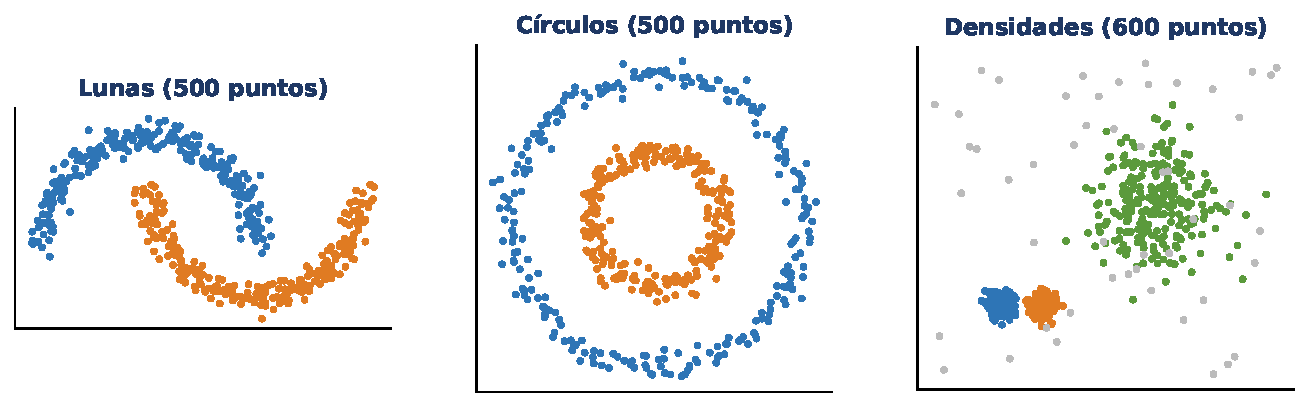
\includegraphics[width=0.95\textwidth]{lab_datos}
  \begin{itemize}
    \item \textbf{Lunas}: dos grupos entrelazados, no convexos.
    \item \textbf{Círculos}: un grupo rodea al otro; ningún centro los separa.
    \item \textbf{Densidades}: dos grupos densos y pegados, uno disperso, y 50 puntos de ruido uniforme.
  \end{itemize}
\end{frame}

\begin{frame}[fragile]{Paso 2: elegir $\eps$ para DBSCAN}
\begin{lstlisting}
for nombre, (X, y) in datos.items():
    d = np.sort(NearestNeighbors(n_neighbors=10).fit(X).kneighbors(X)[0][:, -1])
    plt.plot(d)    # grafica de k-distancia con min_samples = 10
\end{lstlisting}
  \centering
  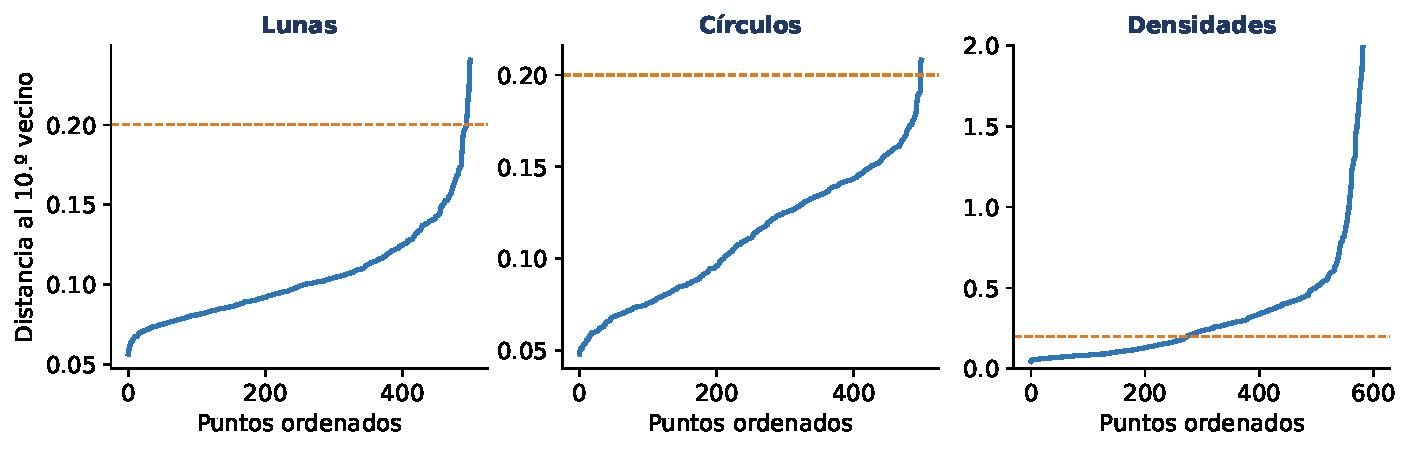
\includegraphics[width=0.9\textwidth]{lab_k_distancia}
  \begin{itemize}
    \item En lunas y círculos el codo está cerca de 0.2: se usa $\eps = 0.2$ y \texttt{min\_samples} $= 10$.
    \item En densidades la curva sube de forma gradual: no hay un codo claro, señal de que las
          densidades son distintas.
  \end{itemize}
\end{frame}

\begin{frame}[fragile]{Paso 3: DBSCAN con densidades distintas}
\begin{lstlisting}
X, y = datos["Densidades"]
for eps in np.arange(0.1, 1.01, 0.05):
    z = DBSCAN(eps=eps, min_samples=10).fit_predict(X)
    print(round(eps, 2), adjusted_rand_score(y, z))
\end{lstlisting}
  \begin{columns}[c]
    \column{0.48\textwidth}
    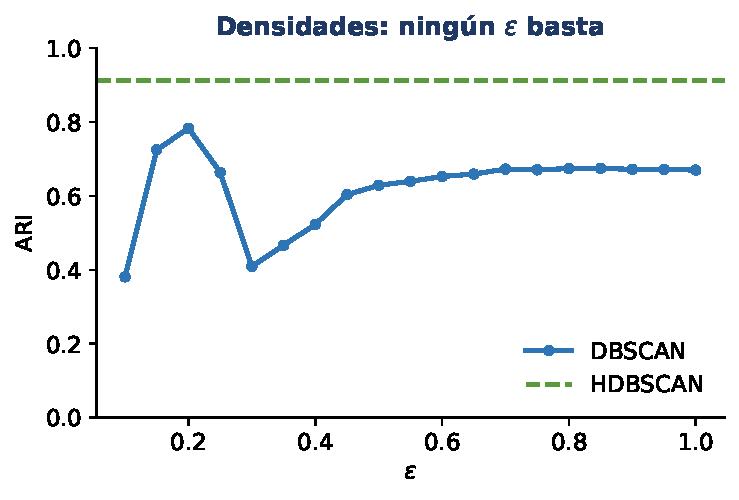
\includegraphics[width=\textwidth]{lab_barrido}
    \column{0.5\textwidth}
    \small
    \begin{itemize}
      \item El mejor DBSCAN obtiene ARI 0.78, con $\eps = 0.2$: separa los dos grupos densos,
            pero 236 de los 250 puntos del disperso quedan como ruido.
      \item Con $\eps \ge 0.35$ los dos densos se unen en un grupo; el disperso aparece, pero con parte de sus puntos como ruido.
      \item HDBSCAN, con \texttt{min\_cluster\_size} $=15$ y sin elegir $\eps$, obtiene 0.91.
    \end{itemize}
  \end{columns}
\end{frame}

\begin{frame}[fragile]{Paso 4: los cuatro métodos en los tres conjuntos}
\begin{lstlisting}
for nombre, (X, y) in datos.items():
    k = len(set(y) - {-1})
    modelos = {"k-medias": KMeans(k, n_init=10, random_state=0),
               "DBSCAN": DBSCAN(eps=0.2, min_samples=10),
               "HDBSCAN": HDBSCAN(min_cluster_size=15),
               "Espectral": SpectralClustering(k, affinity="nearest_neighbors",
                                               n_neighbors=10, random_state=0)}
    for metodo, modelo in modelos.items():
        z = modelo.fit_predict(X)
        print(nombre, metodo, round(adjusted_rand_score(y, z), 2), (z == -1).sum())
\end{lstlisting}
  \vspace{4pt}
  \centering
  \small
  \begin{tabular}{@{}lcccc@{}}
    \toprule
    \textbf{ARI} & \textbf{k-medias} & \textbf{DBSCAN} & \textbf{HDBSCAN} & \textbf{Espectral}\\
    \midrule
    Lunas      & 0.24 & 1.00 & 1.00 & 1.00 \\
    Círculos   & 0.00 & 1.00 & 1.00 & 1.00 \\
    Densidades & 0.46 & 0.78 & 0.91 & 0.85 \\
    \bottomrule
  \end{tabular}
\end{frame}

\begin{frame}{Paso 4: los resultados}
  \begin{columns}[c]
    \column{0.58\textwidth}
    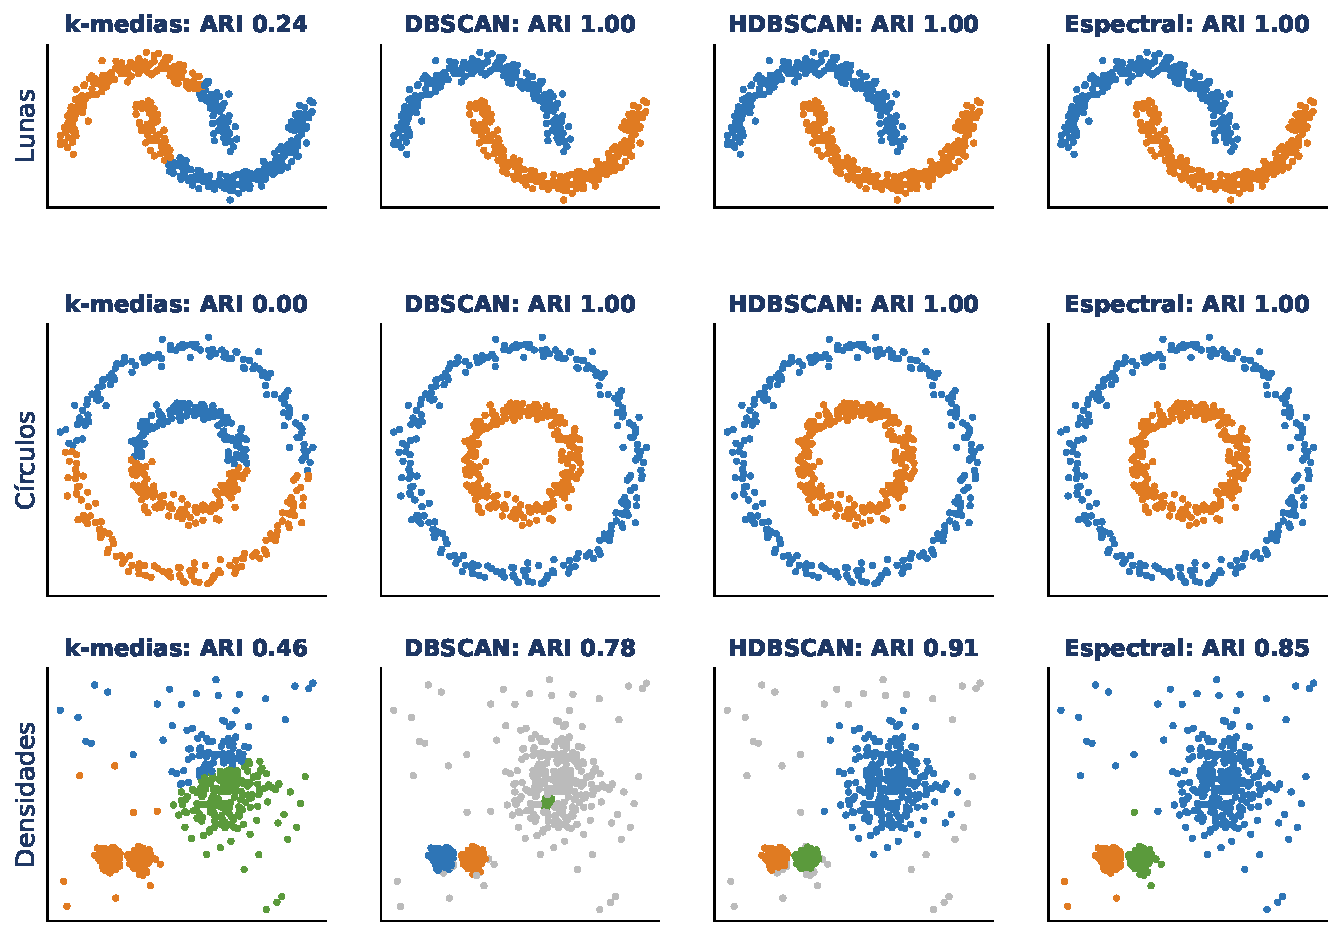
\includegraphics[width=\textwidth]{lab_comparacion}
    \column{0.4\textwidth}
    \small
    \begin{itemize}
      \item Lunas y círculos: los tres métodos no convexos aciertan; k-medias corta las formas.
      \item Densidades, espectral: separa bien los tres grupos, pero asigna los 50 puntos de
            ruido a algún grupo (no tiene etiqueta de ruido).
      \item Densidades, HDBSCAN: marca 47 puntos como ruido; 35 son del ruido inyectado.
            Los otros 15 puntos de ruido quedan junto al grupo disperso y se le asignan.
      \item k-medias divide el grupo disperso y une los dos densos.
    \end{itemize}
  \end{columns}
\end{frame}

\begin{frame}{Conclusiones del laboratorio}
  \begin{itemize}
    \item Con grupos no convexos de densidad parecida (lunas, círculos), DBSCAN, HDBSCAN y espectral
          recuperan los grupos; k-medias no.
    \item La gráfica de k-distancia da un buen $\eps$ cuando tiene un codo claro; si no lo tiene,
          las densidades son distintas y ningún $\eps$ basta.
    \item HDBSCAN resuelve las densidades distintas con un parámetro fácil de interpretar
          (\texttt{min\_cluster\_size}) y además marca el ruido.
    \item El agrupamiento espectral separa bien los grupos, pero necesita $K$ y no detecta ruido.
    \item Los mismos parámetros ($\eps=0.2$, \texttt{min\_samples} $=10$, \texttt{min\_cluster\_size} $=15$,
          10 vecinos) sirvieron en los tres conjuntos porque tienen escalas parecidas; con otros
          datos hay que estandarizar y volver a elegirlos.
  \end{itemize}
\end{frame}

%  El mismo código, ejecutado, está en laboratorio_densidad_espectral.ipynb
% =====================================================================
\section{Laboratorio: densidad y espectral en formas no convexas}
% =====================================================================

\begin{frame}[fragile]{Paso 1: los datos}
\begin{lstlisting}
import numpy as np, pandas as pd
from sklearn.datasets import make_moons, make_circles, make_blobs
from sklearn.cluster import KMeans, DBSCAN, HDBSCAN, SpectralClustering
from sklearn.neighbors import NearestNeighbors
from sklearn.metrics import adjusted_rand_score

Xm, ym = make_moons(500, noise=0.07, random_state=0)
Xc, yc = make_circles(500, factor=0.45, noise=0.05, random_state=0)
Xb, yb = make_blobs([150, 150, 250], centers=[[0, 0], [1.3, 0], [4.5, 3]],
                    cluster_std=[0.2, 0.2, 1.0], random_state=0)
ruido = np.random.default_rng(0).uniform([-2, -2], [8, 7], (50, 2))
Xd, yd = np.r_[Xb, ruido], np.r_[yb, -np.ones(50, int)]   # el ruido tiene etiqueta -1
datos = {"Lunas": (Xm, ym), "Círculos": (Xc, yc), "Densidades": (Xd, yd)}
\end{lstlisting}
  {\small Las etiquetas verdaderas sólo se usan para evaluar con el ARI; el ruido cuenta como una clase más.}
\end{frame}

\begin{frame}{Paso 1: los tres conjuntos}
  \centering
  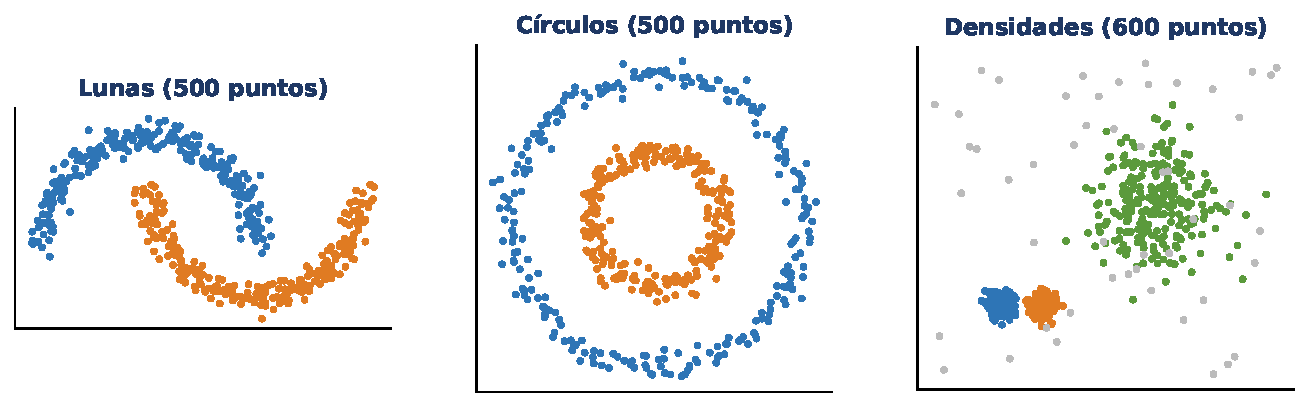
\includegraphics[width=0.95\textwidth]{lab_datos}
  \begin{itemize}
    \item \textbf{Lunas}: dos grupos entrelazados, no convexos.
    \item \textbf{Círculos}: un grupo rodea al otro; ningún centro los separa.
    \item \textbf{Densidades}: dos grupos densos y pegados, uno disperso, y 50 puntos de ruido uniforme.
  \end{itemize}
\end{frame}

\begin{frame}[fragile]{Paso 2: elegir $\eps$ para DBSCAN}
\begin{lstlisting}
for nombre, (X, y) in datos.items():
    d = np.sort(NearestNeighbors(n_neighbors=10).fit(X).kneighbors(X)[0][:, -1])
    plt.plot(d)    # grafica de k-distancia con min_samples = 10
\end{lstlisting}
  \centering
  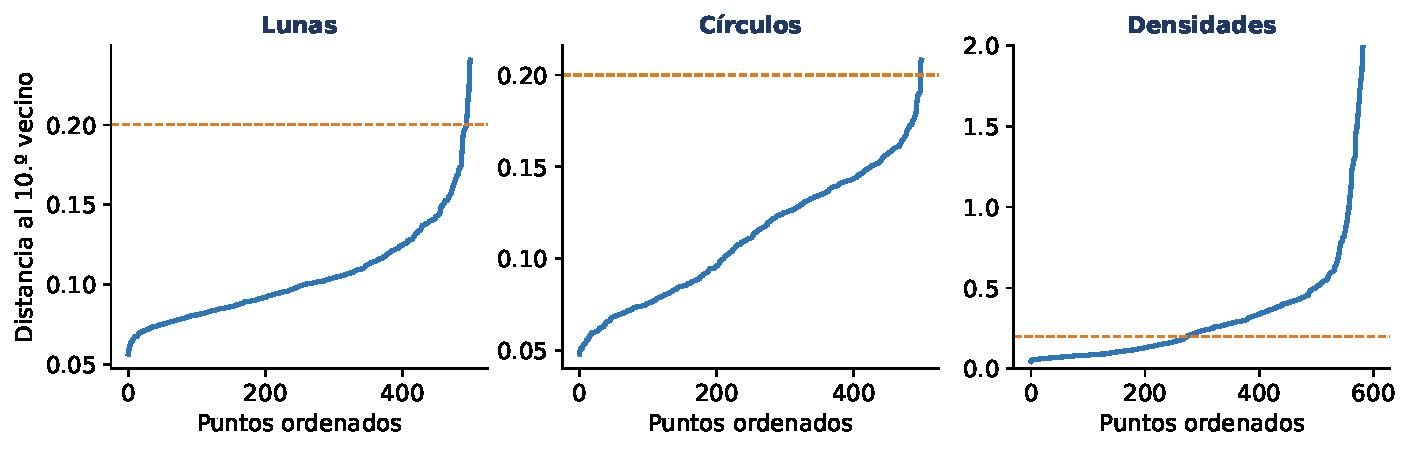
\includegraphics[width=0.9\textwidth]{lab_k_distancia}
  \begin{itemize}
    \item En lunas y círculos el codo está cerca de 0.2: se usa $\eps = 0.2$ y \texttt{min\_samples} $= 10$.
    \item En densidades la curva sube de forma gradual: no hay un codo claro, señal de que las
          densidades son distintas.
  \end{itemize}
\end{frame}

\begin{frame}[fragile]{Paso 3: DBSCAN con densidades distintas}
\begin{lstlisting}
X, y = datos["Densidades"]
for eps in np.arange(0.1, 1.01, 0.05):
    z = DBSCAN(eps=eps, min_samples=10).fit_predict(X)
    print(round(eps, 2), adjusted_rand_score(y, z))
\end{lstlisting}
  \begin{columns}[c]
    \column{0.48\textwidth}
    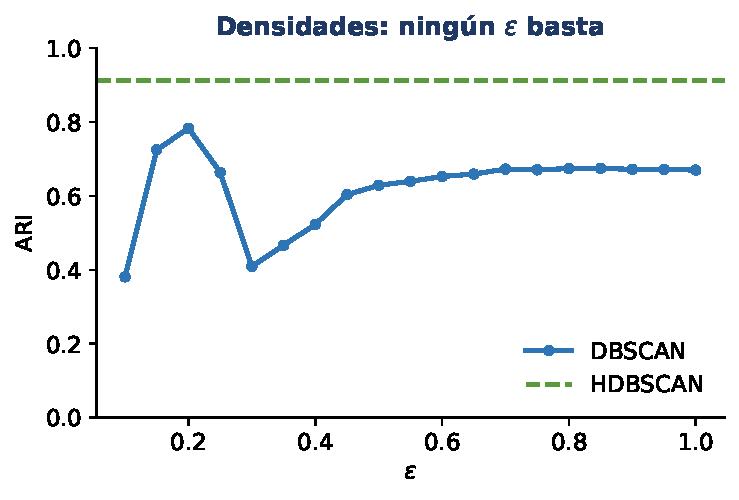
\includegraphics[width=\textwidth]{lab_barrido}
    \column{0.5\textwidth}
    \small
    \begin{itemize}
      \item El mejor DBSCAN obtiene ARI 0.78, con $\eps = 0.2$: separa los dos grupos densos,
            pero 236 de los 250 puntos del disperso quedan como ruido.
      \item Con $\eps \ge 0.35$ los dos densos se unen en un grupo; el disperso aparece, pero con parte de sus puntos como ruido.
      \item HDBSCAN, con \texttt{min\_cluster\_size} $=15$ y sin elegir $\eps$, obtiene 0.91.
    \end{itemize}
  \end{columns}
\end{frame}

\begin{frame}[fragile]{Paso 4: los cuatro métodos en los tres conjuntos}
\begin{lstlisting}
for nombre, (X, y) in datos.items():
    k = len(set(y) - {-1})
    modelos = {"k-medias": KMeans(k, n_init=10, random_state=0),
               "DBSCAN": DBSCAN(eps=0.2, min_samples=10),
               "HDBSCAN": HDBSCAN(min_cluster_size=15),
               "Espectral": SpectralClustering(k, affinity="nearest_neighbors",
                                               n_neighbors=10, random_state=0)}
    for metodo, modelo in modelos.items():
        z = modelo.fit_predict(X)
        print(nombre, metodo, round(adjusted_rand_score(y, z), 2), (z == -1).sum())
\end{lstlisting}
  \vspace{4pt}
  \centering
  \small
  \begin{tabular}{@{}lcccc@{}}
    \toprule
    \textbf{ARI} & \textbf{k-medias} & \textbf{DBSCAN} & \textbf{HDBSCAN} & \textbf{Espectral}\\
    \midrule
    Lunas      & 0.24 & 1.00 & 1.00 & 1.00 \\
    Círculos   & 0.00 & 1.00 & 1.00 & 1.00 \\
    Densidades & 0.46 & 0.78 & 0.91 & 0.85 \\
    \bottomrule
  \end{tabular}
\end{frame}

\begin{frame}{Paso 4: los resultados}
  \begin{columns}[c]
    \column{0.58\textwidth}
    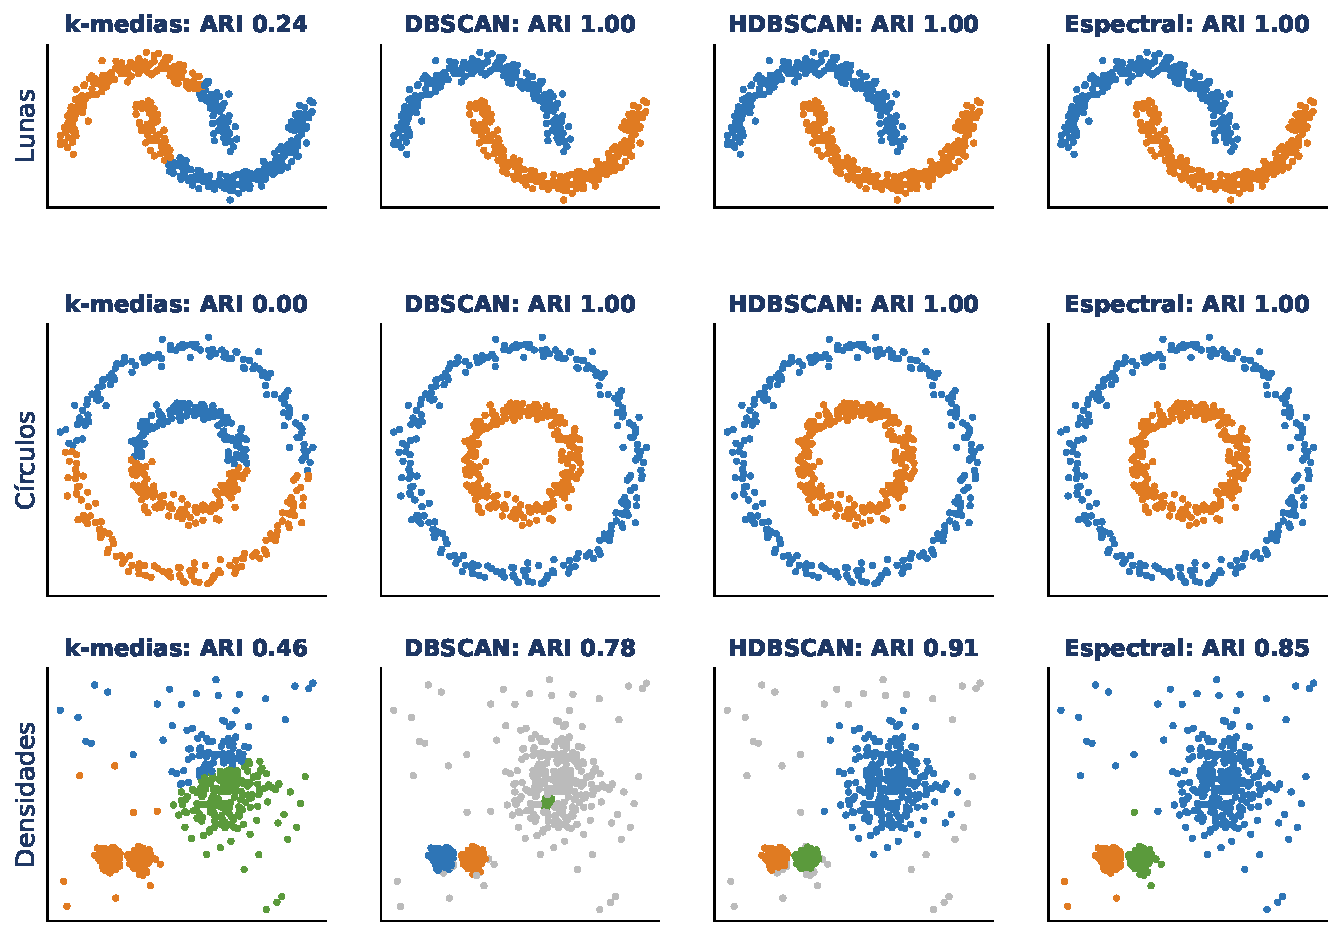
\includegraphics[width=\textwidth]{lab_comparacion}
    \column{0.4\textwidth}
    \small
    \begin{itemize}
      \item Lunas y círculos: los tres métodos no convexos aciertan; k-medias corta las formas.
      \item Densidades, espectral: separa bien los tres grupos, pero asigna los 50 puntos de
            ruido a algún grupo (no tiene etiqueta de ruido).
      \item Densidades, HDBSCAN: marca 47 puntos como ruido; 35 son del ruido inyectado.
            Los otros 15 puntos de ruido quedan junto al grupo disperso y se le asignan.
      \item k-medias divide el grupo disperso y une los dos densos.
    \end{itemize}
  \end{columns}
\end{frame}

\begin{frame}{Conclusiones del laboratorio}
  \begin{itemize}
    \item Con grupos no convexos de densidad parecida (lunas, círculos), DBSCAN, HDBSCAN y espectral
          recuperan los grupos; k-medias no.
    \item La gráfica de k-distancia da un buen $\eps$ cuando tiene un codo claro; si no lo tiene,
          las densidades son distintas y ningún $\eps$ basta.
    \item HDBSCAN resuelve las densidades distintas con un parámetro fácil de interpretar
          (\texttt{min\_cluster\_size}) y además marca el ruido.
    \item El agrupamiento espectral separa bien los grupos, pero necesita $K$ y no detecta ruido.
    \item Los mismos parámetros ($\eps=0.2$, \texttt{min\_samples} $=10$, \texttt{min\_cluster\_size} $=15$,
          10 vecinos) sirvieron en los tres conjuntos porque tienen escalas parecidas; con otros
          datos hay que estandarizar y volver a elegirlos.
  \end{itemize}
\end{frame}

%  El mismo código, ejecutado, está en laboratorio_densidad_espectral.ipynb
% =====================================================================
\section{Laboratorio: densidad y espectral en formas no convexas}
% =====================================================================

\begin{frame}[fragile]{Paso 1: los datos}
\begin{lstlisting}
import numpy as np, pandas as pd
from sklearn.datasets import make_moons, make_circles, make_blobs
from sklearn.cluster import KMeans, DBSCAN, HDBSCAN, SpectralClustering
from sklearn.neighbors import NearestNeighbors
from sklearn.metrics import adjusted_rand_score

Xm, ym = make_moons(500, noise=0.07, random_state=0)
Xc, yc = make_circles(500, factor=0.45, noise=0.05, random_state=0)
Xb, yb = make_blobs([150, 150, 250], centers=[[0, 0], [1.3, 0], [4.5, 3]],
                    cluster_std=[0.2, 0.2, 1.0], random_state=0)
ruido = np.random.default_rng(0).uniform([-2, -2], [8, 7], (50, 2))
Xd, yd = np.r_[Xb, ruido], np.r_[yb, -np.ones(50, int)]   # el ruido tiene etiqueta -1
datos = {"Lunas": (Xm, ym), "Círculos": (Xc, yc), "Densidades": (Xd, yd)}
\end{lstlisting}
  {\small Las etiquetas verdaderas sólo se usan para evaluar con el ARI; el ruido cuenta como una clase más.}
\end{frame}

\begin{frame}{Paso 1: los tres conjuntos}
  \centering
  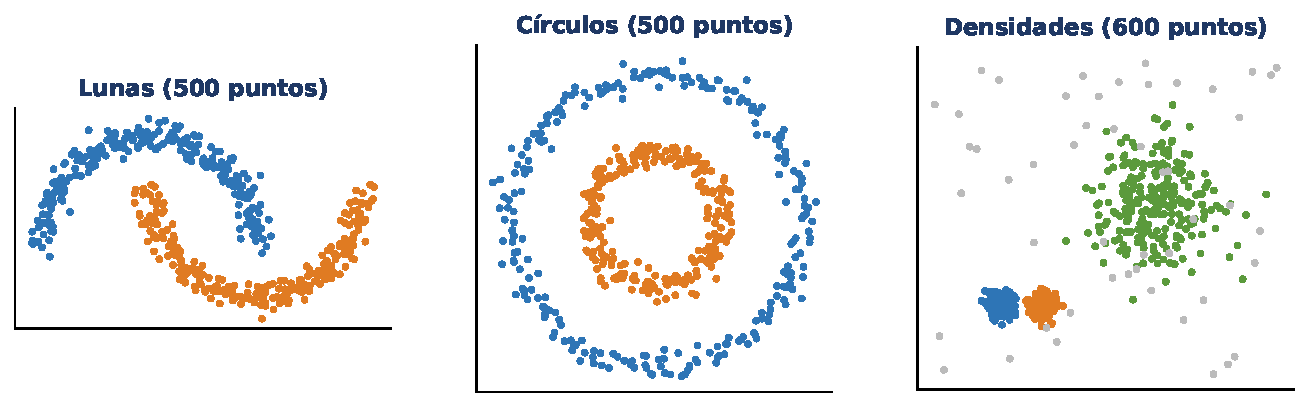
\includegraphics[width=0.95\textwidth]{lab_datos}
  \begin{itemize}
    \item \textbf{Lunas}: dos grupos entrelazados, no convexos.
    \item \textbf{Círculos}: un grupo rodea al otro; ningún centro los separa.
    \item \textbf{Densidades}: dos grupos densos y pegados, uno disperso, y 50 puntos de ruido uniforme.
  \end{itemize}
\end{frame}

\begin{frame}[fragile]{Paso 2: elegir $\eps$ para DBSCAN}
\begin{lstlisting}
for nombre, (X, y) in datos.items():
    d = np.sort(NearestNeighbors(n_neighbors=10).fit(X).kneighbors(X)[0][:, -1])
    plt.plot(d)    # grafica de k-distancia con min_samples = 10
\end{lstlisting}
  \centering
  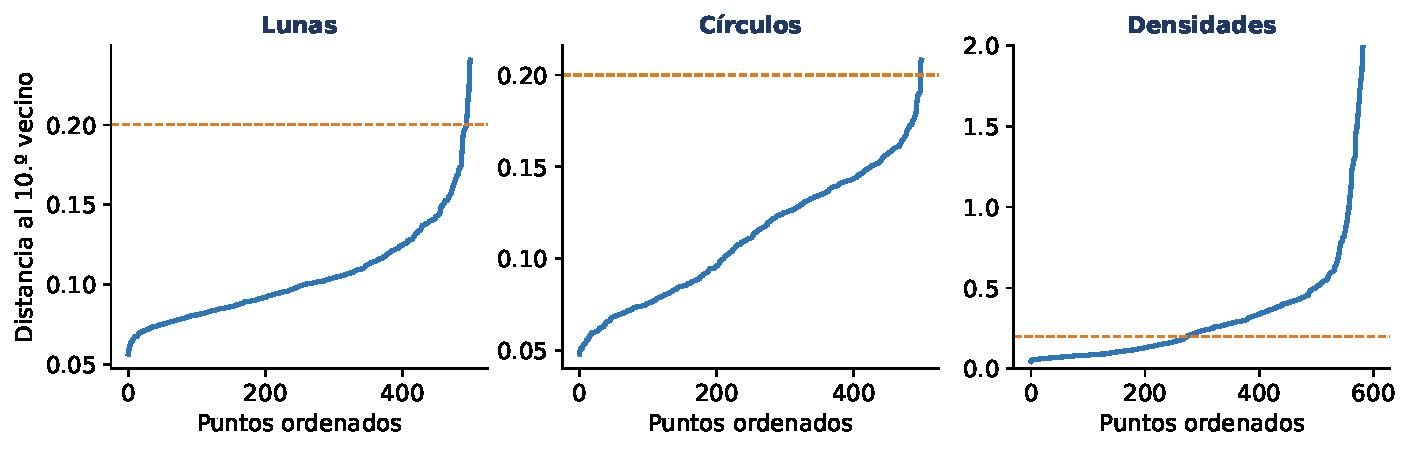
\includegraphics[width=0.9\textwidth]{lab_k_distancia}
  \begin{itemize}
    \item En lunas y círculos el codo está cerca de 0.2: se usa $\eps = 0.2$ y \texttt{min\_samples} $= 10$.
    \item En densidades la curva sube de forma gradual: no hay un codo claro, señal de que las
          densidades son distintas.
  \end{itemize}
\end{frame}

\begin{frame}[fragile]{Paso 3: DBSCAN con densidades distintas}
\begin{lstlisting}
X, y = datos["Densidades"]
for eps in np.arange(0.1, 1.01, 0.05):
    z = DBSCAN(eps=eps, min_samples=10).fit_predict(X)
    print(round(eps, 2), adjusted_rand_score(y, z))
\end{lstlisting}
  \begin{columns}[c]
    \column{0.48\textwidth}
    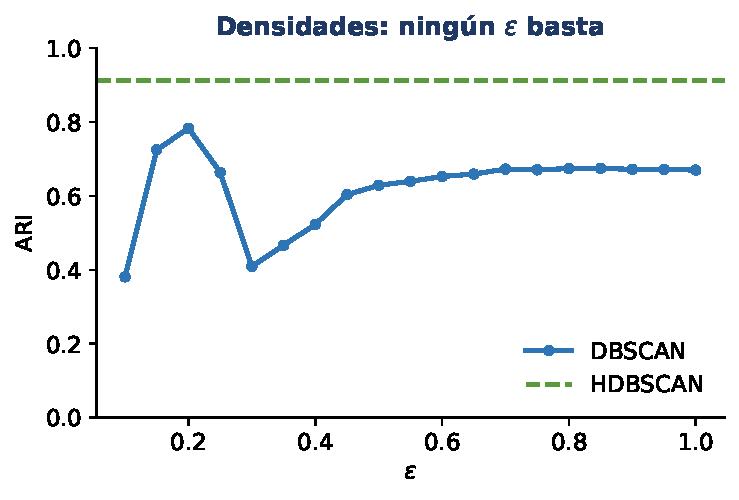
\includegraphics[width=\textwidth]{lab_barrido}
    \column{0.5\textwidth}
    \small
    \begin{itemize}
      \item El mejor DBSCAN obtiene ARI 0.78, con $\eps = 0.2$: separa los dos grupos densos,
            pero 236 de los 250 puntos del disperso quedan como ruido.
      \item Con $\eps \ge 0.35$ los dos densos se unen en un grupo; el disperso aparece, pero con parte de sus puntos como ruido.
      \item HDBSCAN, con \texttt{min\_cluster\_size} $=15$ y sin elegir $\eps$, obtiene 0.91.
    \end{itemize}
  \end{columns}
\end{frame}

\begin{frame}[fragile]{Paso 4: los cuatro métodos en los tres conjuntos}
\begin{lstlisting}
for nombre, (X, y) in datos.items():
    k = len(set(y) - {-1})
    modelos = {"k-medias": KMeans(k, n_init=10, random_state=0),
               "DBSCAN": DBSCAN(eps=0.2, min_samples=10),
               "HDBSCAN": HDBSCAN(min_cluster_size=15),
               "Espectral": SpectralClustering(k, affinity="nearest_neighbors",
                                               n_neighbors=10, random_state=0)}
    for metodo, modelo in modelos.items():
        z = modelo.fit_predict(X)
        print(nombre, metodo, round(adjusted_rand_score(y, z), 2), (z == -1).sum())
\end{lstlisting}
  \vspace{4pt}
  \centering
  \small
  \begin{tabular}{@{}lcccc@{}}
    \toprule
    \textbf{ARI} & \textbf{k-medias} & \textbf{DBSCAN} & \textbf{HDBSCAN} & \textbf{Espectral}\\
    \midrule
    Lunas      & 0.24 & 1.00 & 1.00 & 1.00 \\
    Círculos   & 0.00 & 1.00 & 1.00 & 1.00 \\
    Densidades & 0.46 & 0.78 & 0.91 & 0.85 \\
    \bottomrule
  \end{tabular}
\end{frame}

\begin{frame}{Paso 4: los resultados}
  \begin{columns}[c]
    \column{0.58\textwidth}
    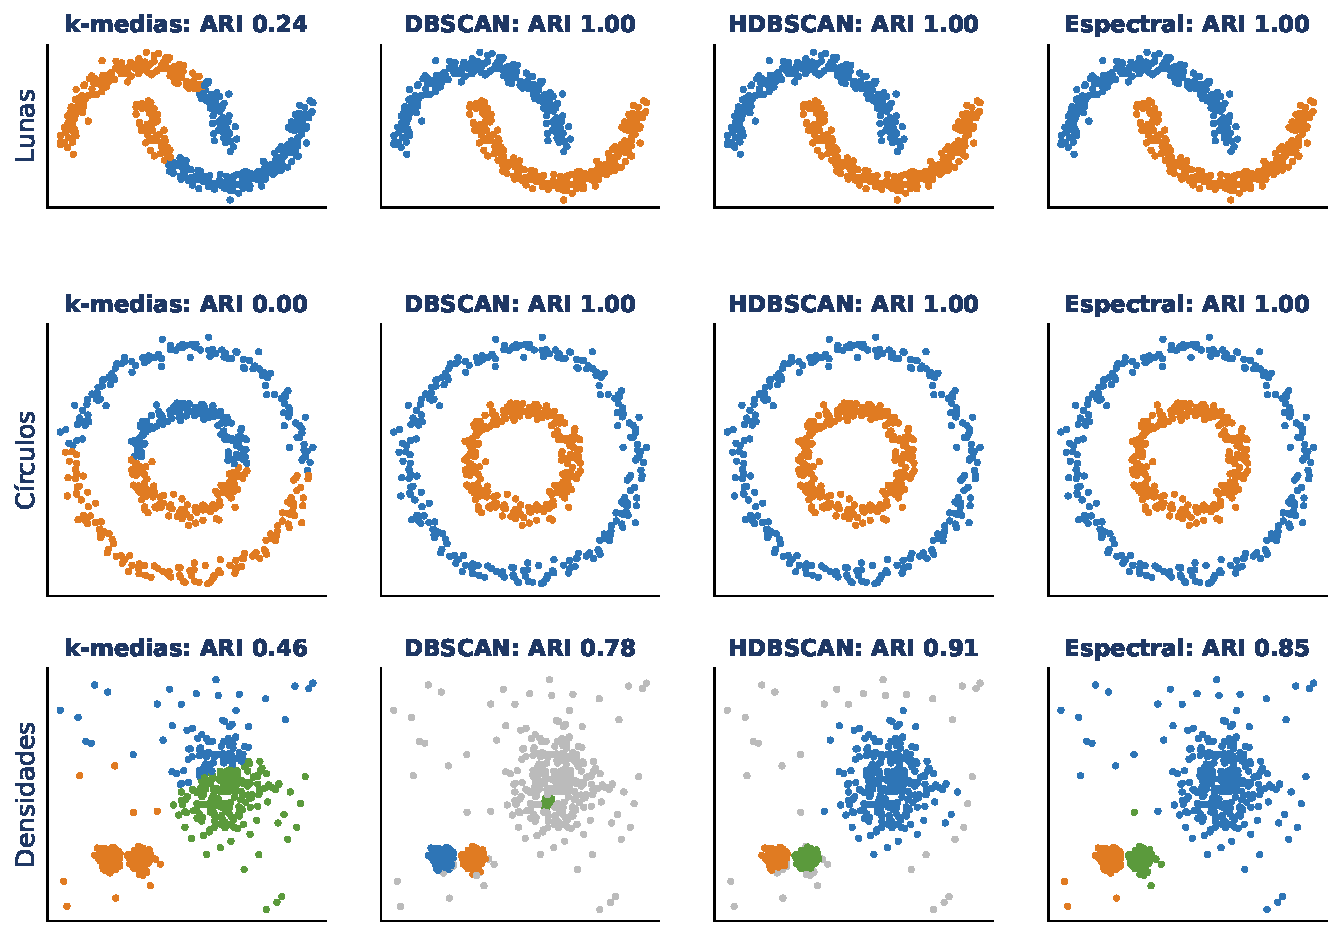
\includegraphics[width=\textwidth]{lab_comparacion}
    \column{0.4\textwidth}
    \small
    \begin{itemize}
      \item Lunas y círculos: los tres métodos no convexos aciertan; k-medias corta las formas.
      \item Densidades, espectral: separa bien los tres grupos, pero asigna los 50 puntos de
            ruido a algún grupo (no tiene etiqueta de ruido).
      \item Densidades, HDBSCAN: marca 47 puntos como ruido; 35 son del ruido inyectado.
            Los otros 15 puntos de ruido quedan junto al grupo disperso y se le asignan.
      \item k-medias divide el grupo disperso y une los dos densos.
    \end{itemize}
  \end{columns}
\end{frame}

\begin{frame}{Conclusiones del laboratorio}
  \begin{itemize}
    \item Con grupos no convexos de densidad parecida (lunas, círculos), DBSCAN, HDBSCAN y espectral
          recuperan los grupos; k-medias no.
    \item La gráfica de k-distancia da un buen $\eps$ cuando tiene un codo claro; si no lo tiene,
          las densidades son distintas y ningún $\eps$ basta.
    \item HDBSCAN resuelve las densidades distintas con un parámetro fácil de interpretar
          (\texttt{min\_cluster\_size}) y además marca el ruido.
    \item El agrupamiento espectral separa bien los grupos, pero necesita $K$ y no detecta ruido.
    \item Los mismos parámetros ($\eps=0.2$, \texttt{min\_samples} $=10$, \texttt{min\_cluster\_size} $=15$,
          10 vecinos) sirvieron en los tres conjuntos porque tienen escalas parecidas; con otros
          datos hay que estandarizar y volver a elegirlos.
  \end{itemize}
\end{frame}
